\documentclass[addpoints,12pt]{exam}

\usepackage{amsmath}
\usepackage{amsthm}
\usepackage{graphicx}
\usepackage{enumitem}
\usepackage{amssymb}
\usepackage{tikz}
\usepackage{multicol}
\usepackage{comment}
\usepackage{geometry}
\usepackage{enumitem}

\printanswers %Remove to hide answers
\pagestyle{headandfoot} %Adds Headers and Footers
\runningheadrule
\firstpageheader{Math 125}{Exam 2 }{\today}
\runningheader{Math 125}
{Exam 2, Page \thepage\ of \numpages}
{\today}
\firstpagefooter{}{\thepage}{}
\runningfooter{}{\thepage}{}

\newcommand{\tft}{
\begin{oneparcheckboxes}
\CorrectChoice True
\choice False
	\end{oneparcheckboxes}
}
\newcommand{\tff}{
\begin{oneparcheckboxes}
\choice True
\CorrectChoice False
	\end{oneparcheckboxes}
	
}
\newcommand{\ynn}{
\begin{oneparcheckboxes}
\choice Yes
\CorrectChoice No
	\end{oneparcheckboxes}
}
\newcommand{\yny}{
\begin{oneparcheckboxes}
\CorrectChoice Yes
\choice No 
	\end{oneparcheckboxes}
}
\checkboxchar{$\Box$}
\checkedchar{$\blacksquare$}

\theoremstyle{definition}
\newtheorem{theorem}{Theorem}

\newtheorem{lemma}{Lemma}
\begin{document}

%The box at the top, and the name
\begin{center}
\fbox{\fbox{\parbox{5.5in}{\centering
Answer the questions in the spaces provided on the
question sheets. If you run out of room for an answer,
continue on the back of the page.}}}
\end{center}
\vspace{0.1in}
\makebox[\textwidth]{Name:\enspace\hrulefill}
\vspace{0.2in}

%Question Formatting
%\qformat{\textbf{Question \thequestion}\quad (\thepoints)\hfill}
%Point Table

%\begin{center}
%\gradetable[h][questions]
%\end{center}

\begin{center}
    \Huge Formulas
\end{center}

\begin{lemma}
    The roots of a polynomial $y = ax^{2}+bx+c$ are given by 
		\[
		x = \frac{-b \pm \sqrt{b^{2}-4ac}}{2a}
		\]
\end{lemma}

\begin{lemma}
    If you would like to find a percent $r$ of a value $P$, you can use the formula 
		\[
		A = Pr
		\]
		If you would like to increase $P$ by a certain percent $r$, you can use 
		\[
		A = P(1+r)
		\]
\end{lemma}

\begin{lemma}
	The simple interest formula is given by 
    \[
    A = P(1+rt)
    \]
		The compound interest formula compounded yearly is given by 
		\[
		A = P(1+r)^{t} 
		\]
		The compound interest formula compounded $n$-times yearly is given by 
		\[
		A = P(1+\frac{r}{n})^{nt}
		\]
		Here $A$ is the amount of money you end with, $P$ is the starting value, $r$ is the rate , and $t$ is the number of years. 
\end{lemma}
\begin{lemma}
	Let $P$ be the amount of a loan at an interest rate $r$, with $n$-payments per year over $t$ years. Then size of the payment is given by 
	\[
	\frac{P(\frac{r}{n})}{\left[1-\left(1+\frac{r}{n}\right)^{-nt}\right]}
	\]
\end{lemma}

\begin{center}
    \Huge Review Questions
\end{center}
%Beginning Questions
\begin{questions}
\question Consider the following list of sentences. Respond Yes if the sentence is a mathematical statement, and No if it is not. 
\begin{enumerate}[label = \alph*)]
	\item \yny The earth is the third planet from the sun.   
	\item \ynn Do your homework. 
	\item \ynn What time does the exam start? 
	\item \yny The ocean does not contain salt water. 
	\item \ynn The Minnesota Vikings are the best football team.  
\end{enumerate}
\question Consider the following statements 
\begin{align*}
	p:  & \text{The dog's name  is Nels.} \\
	q: & \text{Nels has a new toy. } \\
	r: & \text{Nels is at the dog park.} \\
\end{align*}
Write the statement expressed by the symbolic statement in words. 
\begin{enumerate}[label = \alph*)]
    \item $p $ 
		\item $q \wedge r$ 
		\item $\sim r $
		\item $q \leftrightarrow  r $ 
		\item  $q \vee r $
\end{enumerate}
    \begin{enumerate}[label = \alph*)]
        \item The dog's name is Nels. 
				\item Nels has a new toy and Nels is at the dog park. 
				\item Nels is not at the dog park. 
				\item Nels has a new toy if and only if Nels is at the dog park. 
				\item Nels has a new toy or Nels is at the dog park. 
    \end{enumerate}
\question Write the negation of the following statements 
\begin{enumerate}[label = \alph*)]
	\item All people in the class received an $A$ on the exam. 
	\item It is not Monday. 
	\item There exists a jellybean in the candy jar. 
	\item We all live in Yankton. 
	\item Some cats do not like to swim. 
\end{enumerate}
\begin{solution}
    \begin{enumerate}[label = \alph*)]
        \item There exists someone in the class who did not recieve an $A$ on the exam. 
				\item It is Monday. 
				\item All jelly beans are not in the candy jar. 
				\item There exists a person who does not live in Yankton. 
				\item All cats like to swim. 
    \end{enumerate}
\end{solution}
\question Solve the following linear equation 
\[
2(x-3)-2 = 3-3(x+2) 
\]
\begin{solution}
    \begin{align*}
        2(x-3)-2 = 3-3(x+2)\\
				2x-6 - 2 & = 3 -3x-6 \\
				2x-8 & = -3x-3 \\
				2x & = -3x +5 \\
				5x & = 5 \\
				x & = 1 \\
    \end{align*}
\end{solution}
\question The formula 
\[
C = \frac{5}{9}(F-32)
\]
expresses the relationship between Farenheit temperature, $F$, and Celsius temperate $C$. Evaluate the expression at $F = 41$ to find the equivalent temperature at the Celsius scale. 
\begin{solution}
	\begin{solution}
		\begin{align*}
			C &= \frac{5}{9}(41-32)\\
			C & = \frac{5}{9}(9) \\
			C & = 5 \\
		\end{align*}
	\end{solution}
\end{solution}
\question Solve the quadratic equation by factoring 
\[
x^{2}-2x-15 = 0 
\]
\begin{solution}
     \begin{align*}
			 0 & = x^{2}-2x-15 \\
			& = (x-5)(x+3)\\
     \end{align*} 
		 Therefore, $x=5$ and $x = -3$
\end{solution}

\question Solve the following quadratic equation using the quadratic formula. 
\[
x^{2}+5x - 4 = 0 
\]
Do \textbf{NOT} simplify the quadratic formula after applying the quadratic formula. 
\begin{solution}
    \[
    x = \frac{-5\pm \sqrt{5^{2}-4*1*(-4)}}{2}
    \]
\end{solution}
\question Solve and give the solution set by indicating on a number line. 
\[
-4x + 7 \geq -5 
\]
\begin{solution}
    \begin{align*}
			-4x + 7 & \geq -5 \\
			-4x & \geq -12 \\
			x & \leq 3 \\
    \end{align*}
		\begin{center}
		  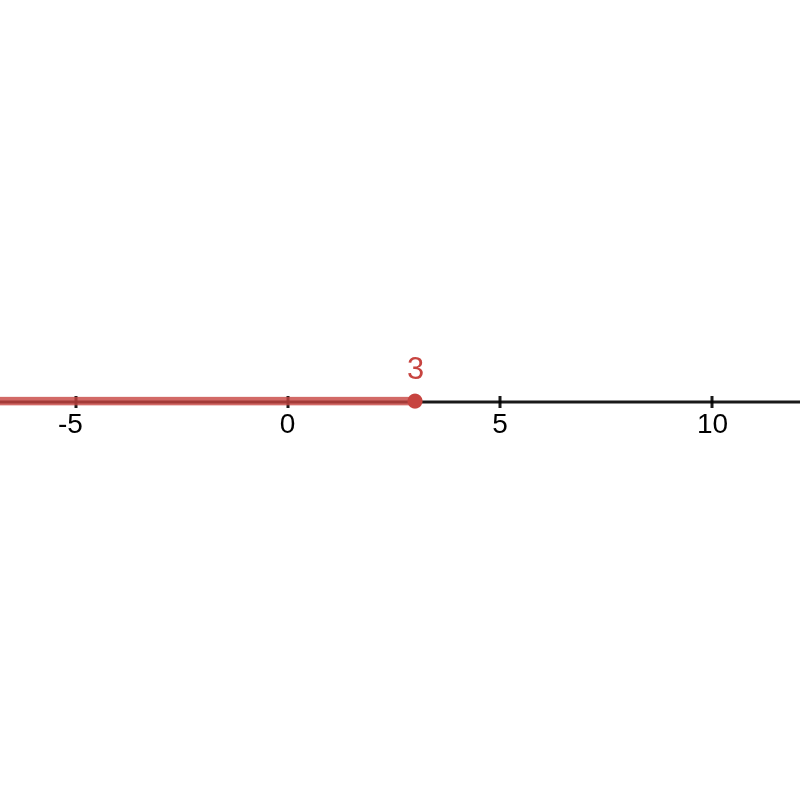
\includegraphics[width=0.6\linewidth]{line.png}
			\end{center}
\end{solution}
\question  You are considering buying a Traeger Grill for your parents for Christmas. The Pro 780 model costs $999.95$ at Ace Hardware. The sales tax at Ace Hardware in Yankton is $6.2\%$. 
\begin{enumerate}[label = \alph*)]
	\item How much sales tax do you pay in total on your purchase? 
	\item What is the total cost of the grill? 
\end{enumerate}
\begin{solution}
    \begin{enumerate}[label = \alph*)]
			\item The amount of sales tax $T$ is given by 
				\[
				T = 999.95 (0.062)
				\]
			\item The total cost of the grill $C$ is given by 
				\[
				C = 999.95 (1.062)
				\]
    \end{enumerate}
\end{solution}\vfill
\question You are looking to invest $2000$ dollars. A bank gives you two options. You can either invest into an account that gives simple interest at $10\%$ per year, or you can invest in an account that makes $8\% $ compound interest. 
\begin{enumerate}[label = \alph*)]
	\item After $4$ years, which account is the better investment? 
	\item After $8$ years, which account is the better investment? 
	\item Which account will be the better investment in the short term? Why is this? 
	\item Which account will be the better investment in the long run? Why is this? 
\end{enumerate}
\begin{solution}
    \begin{enumerate}[label = \alph*)]
			\item The amount after $4$ years with the simple interest is given by 
				\[
				2000 (1+0.1(4)) = 2000*1.4 = 2800
				\]
				The amount after $4$ years with compound interest is given by 
				\[
					2000(1.08)^{4}= \approx 2720.98
				\]
				Therefore the account with simple interest is best after $4$ years. 
				\item The amount after $8$ years with the simple interest is given by 
				\[
				2000 (1+0.1(8)) = 2000*1.8 = 3600
				\]
				The amount after $4$ years with compound interest is given by 
				\[
					2000(1.08)^{8}= \approx 3701.86
				\]
				Therefore the account with compound interest is best after $4$ years. 
			\item The simple interest is better in the short term. After only one year for example, they both calculate interest in the same way, by multiplying by the interest rate. Therefore, the higher interest rate will be better. 
			\item In the long run, the compound interest rate will be better since we take $8\%$ of whatever money we have at a given time. Therefore, once we have more than $2500$ dollars, the compound interest at $8\%$ will make more than the $10\%$ of $2000$ dollars. 
    \end{enumerate}
\end{solution}
    \question Assume that you buy a new car that costs $\$25000$ dollars. You finance it with a $3$ year loan at $4\%$. Assume you make monthly payments. What is the monthly payment for your car loan? 
		\begin{solution}
	    \[
	PMT = \frac{25000(\frac{0.04}{12})}{\left[1-\left(1+\frac{0.04}{12}\right)^{-12*3}\right]}
	    \]
			Which is about $\$738.10$
		\end{solution}
\end{questions}

    
\end{document}
